Un constructor hace escaleras con cada escalón de 28 cm de largo y
elevación de 18 cm, para que la gente no se tropiece. Todas las escaleras tienen un soporte diagonal
que conecta los escalones, como se muestra en la figura \ref{fig:des_pitagoras_02a}:

\begin{figure}[H]
    \begin{center}
        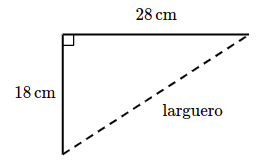
\includegraphics[width=0.3\textwidth]{../images/des_pitagoras_02a.png}
    \end{center}
    \caption{}
    \label{fig:des_pitagoras_02a}
\end{figure}
Cierta escalera tiene 6 escalones, como se muestra en la figura \ref{fig:des_pitagoras_02b}.
\begin{figure}[H]
    \begin{center}
        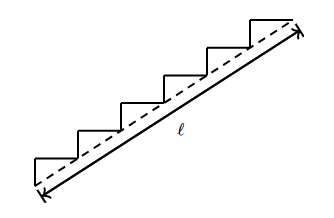
\includegraphics[width=0.3\textwidth]{../images/des_pitagoras_02b.png}
    \end{center}
    \caption{}
    \label{fig:des_pitagoras_02b}
\end{figure}
\textbf{¿Cuál es la longitud $l$ para esta escalera?}\\
\textit{Redondea tu respuesta a la décima de centímetro más cercana.}